\subsection*{Introduction}


De nos jours, la \emph{Vision par ordinateur} et le \emph{Traitement d'Image (PI)} sont omniprésents dans la vie
quotidienne des gens. Il est présent à chaque fois que nous passons devant une caméra de vidéosurveillance, à chaque
fois que nous allons à l'hôpital faire une IRM, à chaque fois que nous conduisons notre voiture et passons devant un
radar et à chaque fois que nous utilisons notre ordinateur, smartphone ou tablette. Il ne peut plus être évité. Les
systèmes utilisant cette technologie sont parfois simples et parfois plus complexes. Aussi, l'usage qui est fait de
cette technologie a de nombreuses finalités telles que l'observation spatiale, le médical, l'amélioration de la qualité
de vie, la surveillance, le contrôle, les systèmes autonome, etc. Désormais, le \emph{Traitement d'images} dispose d'un
large éventail de sujets de recherches et malgré une masse de travaux antérieurs déjà contribués très importante, il
reste encore beaucoup à explorer.

Prenons l'exemple d'une application smartphone moderne qui propose une reconnaissance faciale afin de reconnaître les
personnes qui figurent dans d'une photo. Pour fournir un résultat précis, cette application devra faire beaucoup de
traitements différents en plusieurs étapes. De plus, il y a beaucoup de variables à gérer. Nous pouvons énumérer (non
exhaustivement) la météo, l'exposition lumineuse, la résolution, l'orientation, le nombre de personnes, la localisation
de la personne, la distinction entre les humains et les objets/animaux, etc. Tous ces éléments doivent être
soigneusement manipulés afin de reconnaître enfin la ou les personne(s) figurant dans la photo. Ce que l'application ne
vous dit pas, c'est la complexité de la pipeline de traitement d'image en coulisse  qui, la plupart du temps, ne peut
même pas être exécuté dans son l'intégralité sur son appareil (smartphone, tablette, \ldots). En effet, le traitement
d'images est coûteux en ressources informatiques et ne répondrait pas à la contrainte de temps demandée par
l'utilisateur si l'intégralité du pipeline était exécutée sur l'appareil. Par ailleurs, pour la dernière partie qui est
<< reconnaître la personne sur la photo >>, l'application doit alimenter la photo pré-traitée à un réseau de neurones
formé au préalable par des techniques d'apprentissage en profondeur afin de donner une réponse précise. Il existe des
technologies capables d'intégrer un réseau de neurones dans un téléphone mobile, telles que
MobileNets~\parencite{howard.2017.mobilenets}, mais il reste limité en termes de capacités opérationnelles. Il peut
détecter un être humain à l'intérieur d'une photo, mais ne peut pas dire qui est cet être humain par exemple. C'est
pourquoi les systèmes de réseau neuronaux précis sont généralement hébergés dans le cloud, ce qui ne les rend
disponibles que via Internet. Lors du téléchargement de son image, l'utilisateur n'imagine pas la quantité de
technologies et de puissance de calcul qui va être utilisée pour trouver qui apparaît sur la photo.

Nous comprenons maintenant que, de nos jours, pour créer des applications qui interagissent avec des photos ou des
vidéos, nous devons pouvoir effectuer un traitement d'image précis, rapide et évolutif sur une multitude d'appareils
(smartphone, tablette, \ldots). Afin d'atteindre cet objectif, les traiteurs d'images doivent disposer de deux types
d'outils. Le premier est l'environnement de prototypage, une boîte à outils qui permet au traiteur d'image de
développer, tester et améliorer sa logique applicative. Le second est l'environnement de production qui déploie la
version viable de l'application qui a été développée par le traiteur d'image. Les deux environnements peuvent ne pas
avoir les mêmes besoins. D'une part, l'environnement de prototypage nécessite généralement de disposer d'une boucle de
rétroaction rapide pour les tests et d'une disponibilité des algorithmes des logiciels existants à la pointe des
connaissances actuelles. De cette façon, le traiteur d'image peut facilement construire par-dessus ces briques de base
et être assez rapide pour ne pas attendre longtemps pour obtenir les résultats en testant ses nombreux prototypes.
D'autre part, l'environnement de production doit, lui, être stable, résilient, rapide et évolutif.

Lorsque l'on regarde les standards de l'industrie aujourd'hui, nous remarquons que le langage de programmation
\emph{Python} est le principal choix pour le prototypage. Cependant, Python peut ne pas convenir pour pousser un
prototype viable en production avec un minimum changements par la suite. Nous trouvons qu'il n'est pas idéal que le
traiteur d'image ne puisse pas profiter de nombreuses opportunités d'optimisations, à la fois en termes d'efficacité
algorithmique et à la fois au niveau d'une meilleure utilisation du matériel. Cela serait beaucoup plus efficace d'avoir
des blocs de construction de base de bas niveau qui pourraient être adaptés pour s'adapter à autant de cas d'utilisation
que possible. De cette façon, le traiteur d'image peut facilement s'appuyer sur celles-ci lors de la conception de son
application. Nous distinguons deux types de cas d'utilisation. Le premier concerne la multiplicité des types ou des
algorithmes auxquels le traiteur d'image est confronté. Le deuxième relève de la diversité du matériel sur lequel il
peut vouloir exécuter son programme. L'objectif est d'avoir des blocs de construction qui peuvent être suffisamment
intelligents pour tirer parti des nombreuses opportunités d'optimisation, tant en ce qui concerne les données d'entrée
de types ou d'algorithmes et le matériel cible. Ensuite, le traiteur d'image verrait une importante amélioration des
performances, par défaut, sans devoir ajuster spécifiquement son application. C'est ainsi que le concept de généricité a
été introduit. Il vise à fournir un terrain d'entente sur la façon dont une image doit se comporter lorsqu'elle est
transmise à des algorithmes de base nécessaires pour des applications complexes. De cette façon, en théorie, il suffit
d'écrire l'algorithme une seule fois pour qu'il fonctionne avec n'importe quel type d'image.

Finalement, il est admis qu'il existe une règle concernant les trois points suivants : la généricité, l'efficacité et la
facilité d'utilisation. La règle énonce que l'on ne peut avoir que deux de ces avantages qu'en sacrifiant le troisième.
Si l'on veut être générique et efficace, alors la solution naïve sera très complexe à utiliser avec beaucoup de
paramètres. Si l'on veut qu'une solution soit générique et facile à utiliser, alors elle ne sera pas très efficace par
défaut. Enfin, si l'on souhaite qu'une solution soit simple d'utilisation et efficace alors elle ne sera pas très
générique. Pour illustrer cette règle, nous pouvons trouver des exemples parmi les bibliothèques existantes. Une
bibliothèque notablement générique et efficace en C++ est Boost~\parencite{boost.2021} : elle est également notoirement
connue pour être difficile à utiliser. Les composants tels que Boost.Graph, Boost.Fusion ou Boost.Spirit sont difficiles
à utiliser. Aussi, une bibliothèque qui est générique et facile à utiliser est le parser Json écrit par Niels
Lohmann~\parencite{nlohmann.2021.json} il s'efforce de gérer chaque cas d'utilisation tout en restant très simple à
intégrer et à utiliser en code utilisateur (syntaxe très proche du Json natif en code C++ en fournissant un DSL (Domain
Specific Language)~\parencite{deursen.2000.DSL} pour analyser les constructions C++ en JSON). Cependant, cela a un coût
et ce parser est plus lent qu'un parser Json optimisé pour la performance tel que
simdjson~\parencite{lemire.2021.simdjson} dont le but est de << parser des gigaoctets de JSON par seconde >>. Enfin, il
existe de nombreux exemples de code convivial et efficace qui ne sont pas génériques. Nous pouvons citer
Scikit-image~\parencite{vanderwalt.2014.skimage} et OpenCV~\parencite{bradski.2000.opencv}, faciles à utiliser et
efficace (beaucoup de code SIMD/GPU manuscrit) mais pas générique en raison des choix de conception.

Dans cette thèse, nous avons choisi de travailler sur une bibliothèque de traitement d'images en poursuivant les travaux
sur Pylene~\parencite{carlinet.2018.pylena}. Mais travailler uniquement au niveau de la bibliothèque restreindrait
l'utilisabilité de notre travail et donc son impact. C'est pourquoi nous visons à toucher les utilisateurs mettant au
point des prototypes en fournissant un package qui peut être utilisé par un langage dynamique tel que Python, sans
sacrifier les performances. En particulier, nous visons la disponibilité d'utilisation dans un notebook Jupyter. Un
objectif très important pour nous est d'être utilisable en milieu éducatif, ce qui est une force de Python. Dans cette
bibliothèque, nous montrons comment être générique et performant, tout en restant facile à utiliser. Ce faisant, nous
nous efforçons de casser la règle citée précédemment. Le périmètre de la bibliothèque se limite à la morphologie
mathématique et la fourniture de types d'images versatiles. Nous tirons parti du langage C++ moderne et de ses
nombreuses nouvelles fonctionnalités liées à la généricité et à la performance pour dépasser cette règle dans la zone de
traitement d'image. Enfin, nous tentons, d'apporter les outils et les concepts de bas niveau du monde statique au monde
du prototypage de haut niveau et dynamique pour une meilleure diffusion et facilité d'utilisation, grâce un pont entre
ces deux mondes.

C'est avec cette philosophie à l'esprit que ce manuscrit présente notre travail de thèse lié au langage C++ appliqué au
traitement d'images. Il est organisé comme suit :

\paragraph{Programmation générique (généricité)} Ce chapitre présente l'état de l'art sur la notion de généricité. Nous
expliquons son origine, comment il a évolué au fil du temps (en particulier dans le langage C++), quels problèmes il
résout et quels problèmes il crée. Nous expliquons pourquoi le traitement d'image et la généricité fonctionnent bien
ensemble. Enfin, nous faisons le tour des outils existants qui permettent à la généricité (intrinsèquement restreinte au
langage compilé) d'exister dans le monde dynamique (avec langages interprétés tels que Python).

\paragraph{Taxonomie pour le traitement d'images : types d'images et algorithmes.} Ce chapitre présente notre première
contribution dans le domaine du traitement d'images qui consiste à réaliser une taxonomie complète des différentes
familles d'images ainsi que des différentes familles d'algorithmes. Ce chapitre explique, entre autres, la notion de
concept et son application au domaine du traitement d'image. Nous expliquons comment extraire un concept d'un code
existant et comment l'exploiter pour rendre le code plus efficace et lisible. Nous proposons enfin notre point de vue
sous la forme d'une collection de concepts liés au domaine du traitement d'image.

\paragraph{Les Vues d'Image} Ce chapitre présente notre deuxième contribution qui est une généralisation du concept de
Vue (tiré du langage C++, du travail sur les \emph{ranges}~\parencite{niebler.2018.ranges}) aux images. Cela permet la
création d'images légères et peu coûteuses à copier. Cela permet également d'avoir une approche beaucoup plus simple
pour concevoir un pipeline de traitement d'image en enchaînant opérations directement dans le code de manière intuitive.
Les \emph{ranges} sont le ciment de nouvelles façons de concevoir pour faciliter l'utilisation d'une image dans des
algorithmes qui peuvent donc améliorer leur aspect générique. Enfin, nous discutons du concept d'évaluation paresseuse
et de l'impact des vues sur les performances.

\paragraph{Un pont entre le monde statique et le monde dynamique} Ce chapitre présente notre troisième contribution qui
est un moyen de donner accès aux fonctionnalités génériques d'un langage compilé (tel que C++) à un langage dynamique
(tel que Python) pour faciliter le passage entre la phase de prototypage et la phase de production. En effet, il n'est
vraiment pas évident d'être capable de concilier du code générique de C++ dont la généricité est résolue au moment de la
compilation (nous appelons cela le << monde statique >>), et du code dynamique de Python qui s'appuie sur des packages
binaires pré-compilés (nous appelons cela le << monde dynamique >>), pour parvenir à une communication efficace entre le
code dynamique et la bibliothèque. Nous ne pouvons pas non plus demander de l'utilisateur de fournir et d'utiliser un
compilateur à chaque fois qu'il veut utiliser notre bibliothèque depuis Python. Dans ce chapitre, nous discutons quelles
sont les solutions existantes qui peuvent être envisagées ainsi que leurs avantages et inconvénients. Nous discutons
ensuite de la manière dont nous avons conçu et réalisé une solution hybride pour arriver à faire ce pont entre le monde
statique et le monde dynamique.


\subsection*{Programmation générique (généricité)}


En les langages naturels, nous disons que quelque chose est générique quand il peut répondre à plusieurs objectifs à la
fois, tout en étant un minimum efficace. Par exemple, un ordinateur est un outil générique qui permet de rédiger des
documents, d'accéder à des e-mails, de parcourir Internet, jouer à des jeux vidéo, regarder des films, lire des e-books
etc. En programmation, on dira qu'un outil est générique lorsqu'il peut répondre à plusieurs objectifs. Par exemple, le
compilateur gcc peut compiler plusieurs langages de programmation (C, C++, Objective-C, Objective-C++, Fortran, Ada, D,
Go et BRIG (HSAIL)) ainsi que cibler plusieurs architectures (IA-32 (x86), x86--64, ARM, SPARC, etc.). Désormais, on
peut dire que gcc est un compilateur générique. À ce stade, il est important de noter que même si un outil est considéré
comme générique, il y a une limitation quant à ce que l'outil peut faire et ce qu'il ne peut pas faire. Un compilateur
malgré la prise en charge de nombreuses langues et architectures, ne pourra pas passer un appel téléphonique ou faire un
café. De ce fait, il est important de noter que la généricité est un aspect qui qualifie quelque chose. Dans ce
chapitre, nous étudions les aspects génériques liés aux bibliothèques et aux langages de programmation.

Cette thèse volontaire laisse de côté l'aspect générique lié à l'architecture cible. En effet, savoir écrire et/ou
générer du code capable de s'exécuter sur un large éventail d'architectures matérielles différentes est un domaine de
recherche à lui tout seul et n'est pas l'objet principal de cette thèse. Il est également connu sous le nom de
\emph{informatique hétérogène}. Au lieu de cela, nous allons se concentrer sur les aspects liés à la généricité au
niveau de la bibliothèque et au niveau du langage de programmation.

\paragraph{Généricité au sein des bibliothèques} Elle est décrite par la cardinalité du nombre de cas d'utilisation
qu'elle peut gérer. Les bibliothèques fournissent toujours leurs propres structures de données, pour représenter et
donner un sens aux données que l'utilisateur veut traiter, ainsi que des algorithmes pour traiter ces données et fournir
différents types de résultats. Une bibliothèque sera alors cataloguée comme
\emph{générique}~\parencite{musser.1994.algorithm} lorsque (i) ses structures de données permet à l'utilisateur de
s'exprimer entièrement, sans limitation et lorsque (ii) sa banque d'algorithmes est suffisamment grande pour faire tout
ce que l'utilisateur voudrait faire avec ses données. En réalité, une telle bibliothèque n'existe pas et il y a toujours
des limitations. Étudier ces limites et quelles raisons les motivent est la clé pour comprendre comment les dépasser à
l'avenir, en développant le support de nouveaux matériels et/ou logiciel pour de nouvelles fonctionnalités permettant
plus de généricité.

\paragraph{Généricité dans les langages de programmation} Elle est décrite par la capacité du langage à exécuter le même
code sur une grande quantité de structures de données~\parencite{dehnert.1998.fundamentals}, qu'elles soient natives
(char, int, \ldots) ou définies par l'utilisateur. Il est aujourd'hui primordial qu'un langage de programmation puisse
le faire. En effet, dans un monde où les technologies de l'information sont omniprésentes, la quantité de code écrit par
les développeurs de logiciels est faramineuse. Et il en va de même pour la quantité de bogues et de vulnérabilités de
sécurité. Pouvoir avoir nativement un langage de programmation qui permet de faire \emph{plus} en écrivant \emph{moins}
se traduit mathématiquement par un coût de développement et de maintenance réduit. Les langages de programmation offrent
de nombreuses façons d'atteindre la généricité qui dépendent des spécificités intrinsèques des langages : compilé ou
interprété, natif ou émulé, etc.

Avant d'entrer dans les détails de ce que la généricité implique pour les bibliothèques et les langages de
programmation, il est nécessaire d'introduire un peu de vocabulaire. Le premier terme est la notion de \emph{type}. Un
\emph{type} (ou \emph{type de données}) est un attribut de données qui indique au compilateur ou à l'interpréteur
comment le programmeur a l'intention d'utiliser les données. La grande majorité des langages de programmation prend en
charge les types de données de base (également appelés types primitifs) tels que les nombres entiers, les nombres à
virgules flottantes, les types booléens et les chaînes de caractères (ASCII, Unicode, etc.). Cet attribut de type
définit les opérations qui peuvent être effectuées sur les données, la signification des données ainsi que la taille des
données en mémoire (les données peuvent alors être stockées sur le tas, la pile, etc.). Un type de données fournit un
ensemble de valeurs à partir desquelles une expression (\cad variable, fonction, etc.) peut prendre ces valeurs. Parmi
les langages de programmation, on peut distinguer ceux qui sont dynamiquement typés et ceux qui sont statiquement typés.
Les langages typés statiquement sont ceux dont les variables sont déclarées contenant un type spécifique. Cette variable
ne peut contenir des données d'un autre type dans le champ où elle est déclarée. Les langages de programmation à typage
statique sont Ada, C, C++, Java, Rust, Go et Scala. Des langages à types dynamiques sont ceux dont les variables peuvent
être réassignées avec une valeur de type différent de celui avec lequel elle a été initialement déclarée. Le type de
variable est ensuite modifié dynamiquement pour s'adapter à la nouvelle valeur qu'elle porte. Des langages de
programmation à typage dynamique sont PHP, Python, JavaScript et Perl.

La conséquence de pouvoir dire quel type une variable contient à tout moment (langage à typage statique) est double.
Pour le développeur, il est plus facile de raisonner sur le code et de repérer les bugs. Pour le compilateur, il est
possible de générer un code binaire optimisé spécifiquement pour ce type de données (vectorisation, etc.). La
conséquence de pouvoir transformer les type qu'une variable peut contenir au moment de l'exécution sert principalement à
faciliter le prototypage. Lors de la modification d'un notebook Jupyter, il est très apprécié de ne pas se limiter à un
seul type pour chaque variable déclarée afin de pour pouvoir itérer sur le prototype plus rapidement.

En traitement d'images, une image \(Im\) est définie sur un domaine \(\mathcal{D}\) (qui contient des points) par la
relation \(\forall x \in \mathcal{D}, y = Im(x)\) où \(y\) est la valeur de l'image \(Im\) pour le point \(x\). Cette
définition se traduit toujours par une structure de données complexe lorsqu'elle est transposée dans un langage de
programmation. Cette structure de données doit être consciente de la mémoire tampon contenant les données de l'image
ainsi que des informations sur la taille et les dimensions de l'image. De plus, pour ajouter à la difficulté, les
informations nécessaires pour définir précisément la structure des données ne sont pas toujours connues lors de
l'écriture du code source. En effet, un cas d'utilisation très simple consiste à lire une image dans un fichier pour la
charger en mémoire. Le fichier peut contenir une image de différents types de données et le programme doit toujours
fonctionner correctement. Il y a de multiples approches pour résoudre ce problème, et nous les abordons dans ce
chapitre.

En projetant la notion de généricité au traitement d'images, nous pouvons déduire que nous avons besoin de deux aspects
importants pour être générique. Tout d'abord, nous devons décorréler les structures de données de leur topologie et des
données sous-jacentes des algorithmes. En effet, nous voulons que nos algorithmes supportent autant de structures de
données que possible. Deuxièmement, de nombreux algorithmes partagent le même schéma calculatoire et peuvent donc être
factorisés ensemble.

\begin{figure}[htbp]
  \centering
  \begin{tabular}{cccc}
                                                                           & image 2D
                                                                           & graph    & mesh \\[5pt]
    entrée:                                                                &
    \fbox{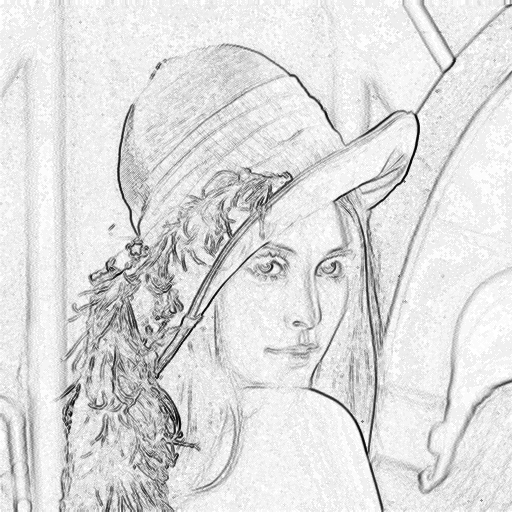
\includegraphics[width=.2\linewidth]{../figures/geninput-000b}}  &
    \fbox{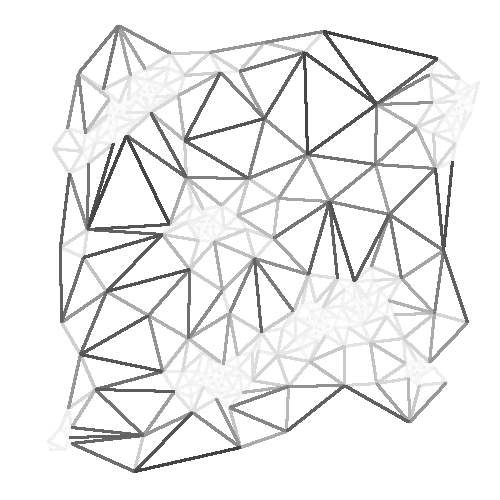
\includegraphics[width=.2\linewidth]{../figures/geninput-001b}}  &
    \fbox{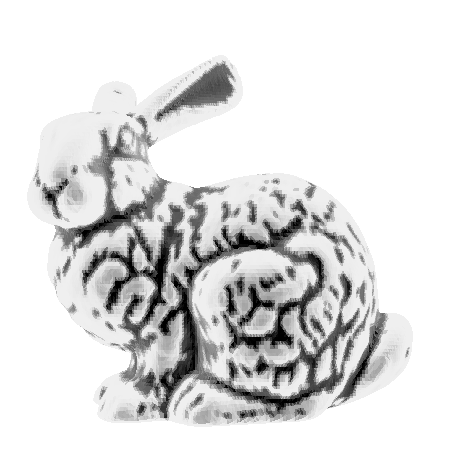
\includegraphics[width=.2\linewidth]{../figures/geninput-002b}}
    \\[5pt]
    %
    sortie:                                                                &
    \fbox{
\includegraphics[width=.2\linewidth]{../figures/genoutput-000}}  &
    \fbox{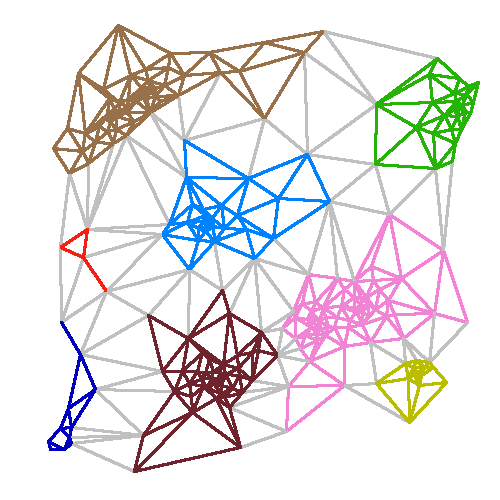
\includegraphics[width=.2\linewidth]{../figures/genoutput-001b}} &
    \fbox{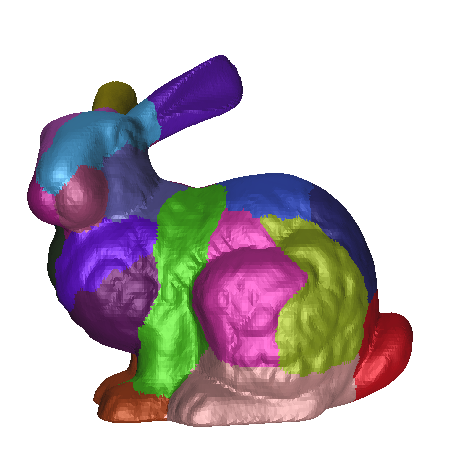
\includegraphics[width=.2\linewidth]{../figures/genoutput-002b}}
    \\
  \end{tabular}
  \bigskip

  \text{Le même code tourne sur toutes ces différentes données d'entrée.}

  \caption[]{Algorithme de ligne de partage des eaux appliqué à trois types d'image différents.}
  \label{summary:fig:type.vs.algo}
\end{figure}

La généricité peut avoir deux significations différentes selon les personnes à qui vous demandez. Par exemple, certaines
diront que la généricité est un aspect haut niveau et qualifie un outil << suffisamment générique >> pour gérer tous ses
cas d'utilisation. D'autres soutiendront que la généricité concerne la façon dont le code est écrit : suffisamment
générique pour gérer tous les cas d'utilisation possibles. Ni l'un ni l'autre n'a tort. Cependant, pour des raisons de
compréhension, nous utiliserons des mots différents pour chacun de ces cas. Un outil assez générique pour gérer un grand
nombre de cas d'utilisation sera appelé \emph{versatile}. Enfin, pour un outil dont le but est de fournir une un
environnement de programmation capable de gérer le code de n'importe quel cas d'utilisation, nous utiliserons le terme
\emph{generic}. Dans cette thèse, la généricité concernera le code. La figure~\ref{summary:fig:type.vs.algo} illustre ce
résultat de la même implémentation générique de l'algorithme de ligne de partage des eaux appliqué sur une image 2D, un
graphe ainsi qu'un maillage.

Dans ce chapitre nous présentons l'origine de la programmation générique, qui remonte
jusqu'à~\citedate[année]{musser.1988.generic} et comment elle a évolué pour être intégrée dans le langage de
programmation Ada puis dans le langage de programmation C++. Ensuite, elle a encore évolué avec la notion de
\emph{concept} qui complétera la boîte à outils nécessaire pour pouvoir pleinement utiliser la programmation générique
sans recourir à des techniques et outils obscurs.

\begin{table}[htbp]
  \centering
  \begin{threeparttable}
    \caption[]{Approches de la généricité: avantages ~\& inconvénients}
    \begin{tabular}[width=0.8\linewidth]{l|ccccc}
      Paradigme                     & VT\tnote{1} & SC\tnote{2} & E\tnote{3} & Une IA\tnote{4} & AE\tnote{5} \\
      \hline
      Duplication de Code           & \cmark      & \xmark      & \cmark     & \xmark          & \xmark      \\
      Généralisation de Code        & \xmark      & \eqmark     & \eqmark    & \cmark          & \xmark      \\
      Programmation Orientée Object & \eqmark     & \cmark      & \xmark     & \cmark          & \cmark      \\
      Programmation Générique:      &             &             &            &                 &             \\
      \quad avec C++11              & \cmark      & \eqmark     & \cmark     & \cmark          & \eqmark     \\
      \quad avec C++17              & \cmark      & \cmark      & \cmark     & \cmark          & \eqmark     \\
      \quad avec C++20              & \cmark      & \cmark      & \cmark     & \cmark          & \cmark      \\
    \end{tabular}
    \begin{tablenotes}
      \item[1] VT: vérification de type.
      \item[2] SC: simplicité du code.
      \item[3] E: efficacité.
      \item[4] Une IA: une seule implémentation par algorithme.
      \item[4] AE: abstraction explicite / généricité contrainte.
    \end{tablenotes}
    \label{summary:table:gen.approaches}
  \end{threeparttable}
\end{table}

Ce chapitre explore les possibilités de réaliser de la programmation générique au sein d'une bibliothèque. En effet, il
y a trois techniques permettant à l'utilisateur d'écrire une seule fois un algorithme de haut niveau pouvant s'exécuter
sur tous les types. Elles sont les approches de \emph{duplication de code}, de \emph{généralisation} et de
\emph{polymorphisme d'inclusion et paramétrique}. Nous présentons dans~\cref{summary:table:gen.approaches} le résultat
de la comparaison de ces approches par rapport aux aspects qui nous intéressent. Nous abordons également les limitations
liées à l'utilisation de ces approches en comparant OpenCV, Scikit-image et Pylene qui utilisent les quatre techniques à
différents niveaux pour atteindre différents objectifs de généricité, de performance et de facilité d'utilisation. De
plus, nous avons identifié des limites liées au type de données sous-jacent, à la structure du domaine et aux
optimisations sur lesquelles nous discuterons des performances via un benchmark concret.

Ce chapitre explore également comment la programmation générique est gérée dans les langages de programmation. Nous
retraçons comment Ada l'a implémenté, et ensuite comment C++ a permis l'expression de clauses contraintes \emph{require}
(concept) dès C++98, même si c'était relativement limitée à cette époque. Nous explorons comment les techniques de
métaprogrammation se sont développées et ont évoluées, en même temps que langage de programmation C++ lui-même, pour
enfin atteindre un point en 2020 (C++20) où il est possible d'écrire des concepts en C++.

Enfin, ce chapitre présente la limitation inhérente aux templates C++, à savoir qu'ils restent dans le monde statique
(moment de la compilation). La généricité (au sens concept C++) n'existe pas dans le binaire final livré à
l'utilisateur. L'utilisateur final, dans son monde dynamique (moment de l'exécution) ne peut pas utiliser un outil
générique (code C++). Nous discutons des différentes approches possibles pour combler cet écart entre le monde statique
(à la compilation) et dynamique (à l'exécution).

Le chapitre suivant fera un large usage de la généricité pour présenter la première contribution de cette thèse : une
taxonomie des notions liées au traitement d'images.


\subsection*{Taxonomie pour le traitement d'images : types d'images et algorithmes}


Dans cette thèse, nous avons poursuivi la recherche sur la façon d'appliquer toutes ces nouvelles fonctionnalités
génériques du langage C++ dans la zone de traitement d'image. Cela nous permet de les tester de manière pratique sur
notre zone de prédilection tout en nous souvenant de nos travail passé, à la fois les succès et les échecs en la
matière. Cependant, comme nous l'avons vu dans le chapitre précédent (Programmation générique (généricité)), faire
naître des concepts à partir du code est quelque chose qui se fait de manière émergente. Désormais, les premiers travaux
seront être de faire un inventaire de tous les algorithmes d'images existants ainsi qu'un inventaire de tous les
algorithmes de traitement d'images (les deux basiques et plus complexes) auxquels nous pouvons penser. De cette façon,
nous remarquerons des modèles de comportement émergeant de types d'images similaires ou algorithmes similaires. Nous
pourrons alors extraire des schémas comportementaux de cet inventaire afin de produire un bilan complet taxonomie sous
la forme d'un cadre de concepts liés au traitement d'images. Ce chapitre est structuré comme suit. Dans un premier
temps, nous étudierons comment extraire un schéma comportemental d'un algorithme simple afin de le raffiner en un ou
plusieurs notions. Dans un second temps nous étudierons la théorie des types d'images, leurs conjonctions, disjonctions.
Nous produirons également un inventaire des algorithmes de traitement d'images limités aux morphologies mathématiques
que nous pouvons exploiter pour la version finale étape. Troisièmement, nous étudierons la généricité intrinsèque des
algorithmes pour produire des canevas tirant parti des propriétés. Enfin, nous étudierons ensuite les schémas
comportementaux liés à l'inventaire sous la forme d'une taxonomie indexant un cadre de concepts sur le traitement
d'images.

Dans ce chapitre, nous présentons que les concepts ne sont pas conçus après des structures de données mais après des
algorithmes. En effet, une notion consiste à extraire un schéma comportemental cohérent d'un bout de code (algorithme)
et à le nommer pour lui donner plus signification. A travers un exemple simple mais concret, nous présentons de manière
didactique comment extraire des concepts d'une image algorithme de traitement (correction gamma).
